\paragraph{Versuchziel}
Aufbau eines Pumpstandes zur Bestimmung der Evakuierungskurve und Durchführung einer 
Leckratenmessung für eine Drehschieberpumpe und eine Turbomolekularpumpe 
(Im Folgenden auch Turbopumpe). Daraus soll später das effektive Saugvermögen bestimmt und in 
Abhängigkeit des Drucks dargestellt werden. Begleitend zum Versuch sollen die Grundlagen der 
Vakuumphysik erarbeitet werden. Zudem soll man sich mit den Komponenten der Vakuumtechnik 
vertraut machen. Weshalb in der Theorie \ref{sec:Theorie} auch Themen zur allgemeinen 
Vakuumphysik  bzw. Vakuumtechnik besprochen werden.
\section{Theorie}
\label{sec:Theorie}
\subsection{Allgemeine Begriffserklärung}
So lange keine ausdrückliche Quellenangebe geben ist, wurde in diesem Kapitel 
Quelle \cite{pfeiffer} verwendet.
\paragraph{Definition des Vakuums}
Umgangssprachlich herrscht ein Vakuum in einem Raum, wenn der Druck im Raum kleiner ist als der 
Atmosphärendruck (\SI{1013}{\hecto\pascal}). Nach DIN-Norm herrscht ein Vakuum, wenn 
die Teilchenzahl außerhalb größer ist als Innen oder der Druck unter \SI{300}{\milli\bar} ist.
\paragraph{Druck}
Druck ist Kraft pro Fläche. Übliche Einheiten sind Pa ,Bar ,Torr und 
Psi. Dabei ist ein hPa = 100 Pa = $ 1\cdot10^{-3}$ Bar = 0,75 Torr = $1,45\cdot10^{-2}$ psi.
\paragraph{Mittlere freie Weglänge}
Die mittlere Weglänge ist die Strecke, die ein Gasteilchen ohne Stoß mit anderen Teilchen 
zurücklegen kann. 
\paragraph{Druckbereiche}
Es lassen sich einige Vakuumbereiche definieren, je nachdem wie stark der Unterdruck ist, ein paar 
davon sind in der Tabelle \ref{tab:db} abgebildet.
\begin{table}
  \centering
  \caption{Druckbereiche der Vakuumbereiche.}
  \resizebox{\textwidth}{!}{%
  \begin{tabular}{c S@{\qquad -}S S@{\qquad-} S S@{\qquad-} S}
    \toprule
     $\text{Druckbereich}$ &
     \multicolumn{2}{c}{$\text{Druck in}\; \si{\hecto\pascal}$}  & 
     \multicolumn{2}{c}{$\text{Teilchen pro}\;  \si{\cubic\meter} $}& 
     \multicolumn{2}{c}{$\text{Mittlere freie Weglänge in}\;  \si{\meter} $} \\
    \midrule
    Grobvakuum & 300 & 1 & 1e19 & 1e16 & 1e-8 & 1e-4 \\
    Feinvakuum & 1&1e-3&1e16 &1e13&1e-4&1e-1\\
    Hochvakuum &	1e-3&1e-7&	1e13&1e9 &1e-1&1e3 \\
    Ultrahochvakuum & 	1e-7&1e-12 &	1e9&1e4&	1e3&1e8 \\
    \bottomrule
  \end{tabular}
}
  \label{tab:db}
\end{table}

\paragraph{Ideales Gas (Nach Quelle \cite{wiki:IG})}
Das \textit{ideale Gas} ist eine Modellvorstellung, die benutzt wird um Gase zubeschreiben. 
Das Modell setzt vorraus, dass die Teilchen miteinander nur durch den elastischen Stoß 
wechselwirken und auch mit den Wänden elastisch Stoßen.
Dann lässt sich die ideale Gasgleichung 
\begin{equation}
pV = n\symup{R}T 
\label{eq:IG} 
\end{equation}
aufstellen, die den Zusammenhang von Druck $p$, Volumen $V$ und Temperatur $T$ darstellt. Dabei 
bezeichnet $n$ die Stoffmenge des betrachteten Gases und $R$ die allgemeine Gaskonstante. 
Ein Spezialfall der idealen Gasgleichung ist das \textit{Gesetz von Boyle-Mariotte} das 
besagt, dass bei konstanter Temperatur der Zusammenhang 
\begin{equation*}
p \approx V^{-1}
\end{equation*}
gilt.
\paragraph{Laminare Strömung}
Bei laminarer Strömung strömen die Teilchen in gleichen zueinander parallelren Strömungsschichten. 
Es tretten keine Verwirbelung, also keine turbulente Strömung, auf. Ob eine turbulente oder 
eine laminare Strömung vorliegt lässt sich mit der Reynoldszahl bestimmen:
\begin{equation*}
\symup{Re} = \frac{\rho \cdot v \cdot l}{\eta} \; .
\end{equation*}
Dabei bezeichnet $\rho$ die Dichte des Fluids, $v$ die Strömungsgeschwindigkeit, $l$ die 
charakteristische Länge und $\eta$ die Dynamische Viskosität des Fluids. Ist 
$ \symup{Re} < 2.300 $ ist die Strömung laminar.

\paragraph{Molekulare Strömung}
Molekulare Strömung herrscht, wenn die mittlere frei Weglänge so groß ist gegen den Strömungskanals, 
dass praktisch keine Wechselwirkung mehr zwischen Teilchen statt findet. Molkeulare Strömung ist 
in der Regel im Bereich des Hoch- und Ultravakuum vorzufinden.

\paragraph{Adsorption (Nach Quelle \cite{wiki:ads})}
Die Anreicherung von Stoffen aus Gasen und/oder Flüssigkeiten an Oberflächen von Festkörpern 
bezeichnet man als Adsorption. Dabei befindet sich das Gas oder die Flüssigkeit im Allgemeinen 
im Übergang zwischen zwei Phasen. 

\paragraph{Absorption (Nach Quelle \cite{wiki:abs})}
Die Aufnahme eines Atoms, Moleküls oder Ions in einer anderen Phase, in das freie Volumen der 
absorbierenden Phase, bezeichnet man als Absorption. Es handelt sich hier also nicht nur 
um eine Anlagerung an der Oberfläche, wie bei der Adsorption.

\paragraph{Desorption}
Ist die Abgabe von Gasmolekühle, die sich vorher durch Ab- und Absorption an Flächen abgereichert 
haben. Dies führt beim Anlegen eines Vakuums, zu einem Gasanfall im Rezipienten (= Raum in dem 
das Vakuum herrschen soll).

\paragraph{Diffusion (Nach Quelle \cite{wiki:dif})}
Ist der Ausgleich zwischen Konzentrationsunterschiede aufgrund der brownschen Molekularbewegung. 
In der Vakuumphysik tritt dieses Phänomen ebenfalls als Gasanfall im Rezipienten auf, wenn 
ein Vakuum angelegt ist.
\paragraph{Virtuelle Lecks (Nach Quelle \cite{wiki:vl})}
Virtuelle Lecks haben ähnliche Effekte wie reale Lecks. Sie entstehen durch Diffusion, Desorption 
aus den Wänden des Rezipienten (z.B. aus Gaseinschlüssen in Schweißnähten) oder durch Rückstände 
von der Fertigung.

\subsection{Vakuumtechnik}
\paragraph{Vakuumpumpe (Nach \cite{pfeiffer})}
In der Vakuumtechnik unterscheidet man zwischen gasfördernen und gasbindenen Pumpen. Die 
gasfördernen Pumpen werden nocheinmal unterschieden in Verdrängerpumpen und kinetische Vakuumpumpen. 
Verdrängerpumpen evakuieren den Rezipienten indem sie das Gas herrausfördern. Kinetische 
Vakuumpumpen befördern das Gas entweder durch Beschleunigung der Gasteilchen in Pumprichtung oder 
durch einen Dampfstrahl, der dann kondensiert wird. Gasbindende Pumpen binden das Gas durch 
Physisorption, Abkühlung auf niedrige Temperaturen oder Chemisorption an Oberflächen.
Die in diesem Versuch verwedeten Vakuumpumpe sind beide gasfördernde Pumpen. Wobei 
die verwedete Drehschieberpumpe eine Verdrängervakuumpumpe ist und die Turbomolekularpumpe 
eine kintetische Vakuumpumpe ist.



\begin{figure}
  \centering
  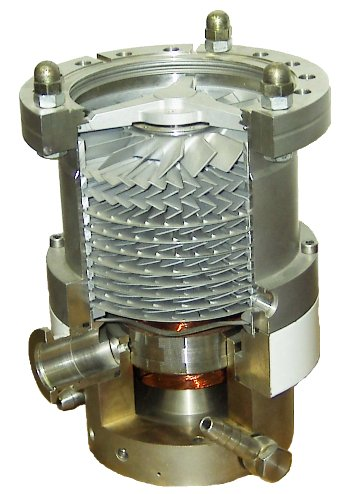
\includegraphics[height = 7cm]{pics/tm.jpg}
  \caption{Schnitt durch eine Turbomolekularpumpe aus Quelle \cite{wiki:tm}.}
  \label{fig:stm}
\end{figure}


